%% Submissions for peer-review must enable line-numbering
%% using the lineno option in the \documentclass command.
%%
%% Preprints and camera-ready submissions do not need
%% line numbers, and should have this option removed.
%%
%% Please note that the line numbering option requires
%% version 1.1 or newer of the wlpeerj.cls file, and
%% the corresponding author info requires v1.2

\documentclass[fleqn,10pt,lineno]{wlpeerj} % for journal submissions

% ZNK -- Adding headers for pandoc

\setlength{\emergencystretch}{3em}
\providecommand{\tightlist}{
\setlength{\itemsep}{0pt}\setlength{\parskip}{0pt}}
\usepackage{lipsum}
\usepackage[unicode=true]{hyperref}
\usepackage{longtable}


% Pandoc syntax highlighting
% See https://github.com/rstudio/rticles/issues/182

\newlength{\cslhangindent}
\setlength{\cslhangindent}{1.5em}
\newenvironment{cslreferences}%
  {\setlength{\parindent}{0pt}%
  \everypar{\setlength{\hangindent}{\cslhangindent}}\ignorespaces}%
  {\par}

% Pandoc Header
\usepackage{lipsum}


\title{Archaeological journals}

\author[1]{Alain Queffelec}

\corrauthor[1]{Alain Queffelec}{\href{mailto:alain.queffelec@u-bordeaux.fr}{\nolinkurl{alain.queffelec@u-bordeaux.fr}}}
\author[1]{Frédéric Santos}

\author[2]{Doug Rocks-Macqueen}


\affil[1]{UMR5199 CNRS PACEA, Univ. Bordeaux, Ministère de la Culture, F-33615 Pessac}
\affil[2]{XXXXXXXXXXXXXXXXX}


%
% \author[1]{First Author}
% \author[2]{Second Author}
% \affil[1]{Address of first author}
% \affil[2]{Address of second author}
% \corrauthor[1]{First Author}{f.author@email.com}

% 

\begin{abstract}
The abstract of the article. It can also be on \emph{multiple} lines.
% Dummy abstract text. Dummy abstract text. Dummy abstract text. Dummy abstract text. Dummy abstract text. Dummy abstract text. Dummy abstract text. Dummy abstract text. Dummy abstract text. Dummy abstract text. Dummy abstract text.
\end{abstract}

\begin{document}

\flushbottom
\maketitle
\thispagestyle{empty}

\hypertarget{introduction}{%
\section*{Introduction}\label{introduction}}
\addcontentsline{toc}{section}{Introduction}

Blablabla

\hypertarget{some-examples}{%
\section*{\texorpdfstring{Some \LaTeX{} Examples}{Some  Examples}}\label{some-examples}}
\addcontentsline{toc}{section}{Some \LaTeX{} Examples}

Use section and subsection commands to organize your document. \LaTeX{} handles all the formatting and numbering automatically. Use ref and label commands for cross-references.

\hypertarget{figures-and-tables}{%
\subsection*{Figures and Tables}\label{figures-and-tables}}
\addcontentsline{toc}{subsection}{Figures and Tables}

Use the table and tabular commands for basic tables --- see Table \ref{tab:widgets}, for example. You can upload a figure (JPEG, PNG or PDF) using the project menu. To include it in your document, use the includegraphics command as in the code for Figure \ref{fig:view} below.

\begin{figure}
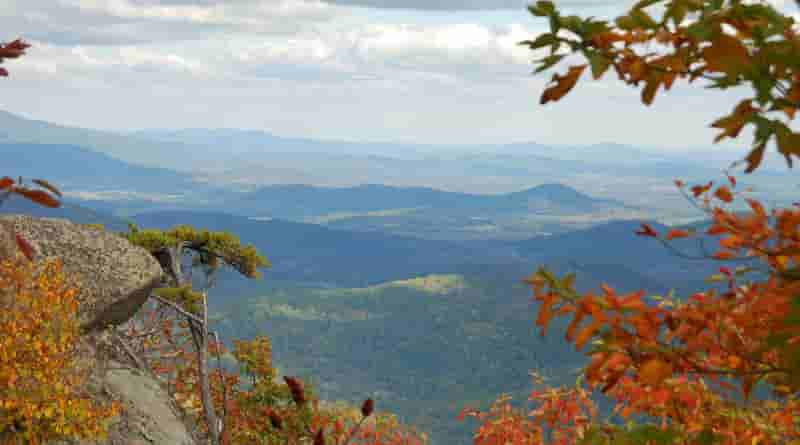
\includegraphics[width=1\linewidth]{view} \caption{An example image.}\label{fig:view}
\end{figure}

\begin{longtable}[]{@{}lr@{}}
\caption{\label{tab:widgets} An Example Table.}\tabularnewline
\toprule
Item & Quantity\tabularnewline
\midrule
\endfirsthead
\toprule
Item & Quantity\tabularnewline
\midrule
\endhead
Widgets & 42\tabularnewline
Gadgets & 13\tabularnewline
\bottomrule
\end{longtable}

\hypertarget{citations}{%
\subsection*{Citations}\label{citations}}
\addcontentsline{toc}{subsection}{Citations}

LaTeX formats citations and references automatically using the bibliography records in your .bib file, which you can edit via the project menu. Use this command for an inline citation, like Pourret et al. (2020) , and the this command for a citation in parentheses (Pourret et al. 2020).

\hypertarget{lists}{%
\subsection*{Lists}\label{lists}}
\addcontentsline{toc}{subsection}{Lists}

You can make lists with automatic numbering \dots

\begin{enumerate}
\def\labelenumi{\arabic{enumi}.}
\tightlist
\item
  Like this,
\item
  and like this.
\end{enumerate}

or bullet points\ldots{}

\begin{itemize}
\tightlist
\item
  Like this,
\item
  and like this.
\end{itemize}

or with descriptions\ldots{}

\begin{itemize}
\tightlist
\item
  \textbf{Word} Definition
\item
  \textbf{Concept} Explanation
\item
  \textbf{Idea} Text
\end{itemize}

We hope you find write\LaTeX~useful for your PeerJ submission, and please let us know if you have any feedback. Further examples with dummy text are included in the following pages.

\hypertarget{methods}{%
\section*{Methods}\label{methods}}
\addcontentsline{toc}{section}{Methods}

\paragraph{Example}

Creation of the initial database by Doug? What was the method? Year? And after that, update of this database in 2021. \textbf{All data for journals not indexed in DOAJ were acquired manually}

\paragraph{}

Extraction of journals from the DOAJ by searching in the keywords ``archaeo'', ``archeo'', ``prehist'' and ``anthropo''. For this last term, we checked it was effectively physical/biological/evolutionary anthropology.

\paragraph{}

Method for JIF, CiteScore etc. ?

\hypertarget{results}{%
\section*{Results}\label{results}}
\addcontentsline{toc}{section}{Results}

\hypertarget{article-processing-charges-and-journal-impact-factor}{%
\subsection*{Article processing charges and journal impact factor}\label{article-processing-charges-and-journal-impact-factor}}
\addcontentsline{toc}{subsection}{Article processing charges and journal impact factor}

\begin{itemize}
\tightlist
\item
  Graphic bars distribution of APC for all journal having gold OA option (including APC = 0\$)
\item
  Plot APC x JIF
\end{itemize}

\emph{Journal figures:}

\begin{itemize}
\tightlist
\item
  Journal Impact Factor (JIF) which is calculated on the two last complete years\\
\item
  5 year JIF: same but on 5 years
\item
  Scopus CiteScore = JIF over 4 years (standard JIF is 2 years) (\url{https://service.elsevier.com/app/answers/detail/a_id/14880/supporthub/scopus/})
\item
  Scopus SCImago Journal Rank (SJR) integrate the prestige of the citation's journal ! (\url{https://service.elsevier.com/app/answers/detail/a_id/14883/supporthub/scopus/}
\item
  Source Normalized Impact per Paper (SNIP) (\url{https://service.elsevier.com/app/answers/detail/a_id/14884/supporthub/scopus/related/1/})
\end{itemize}

\begin{figure}
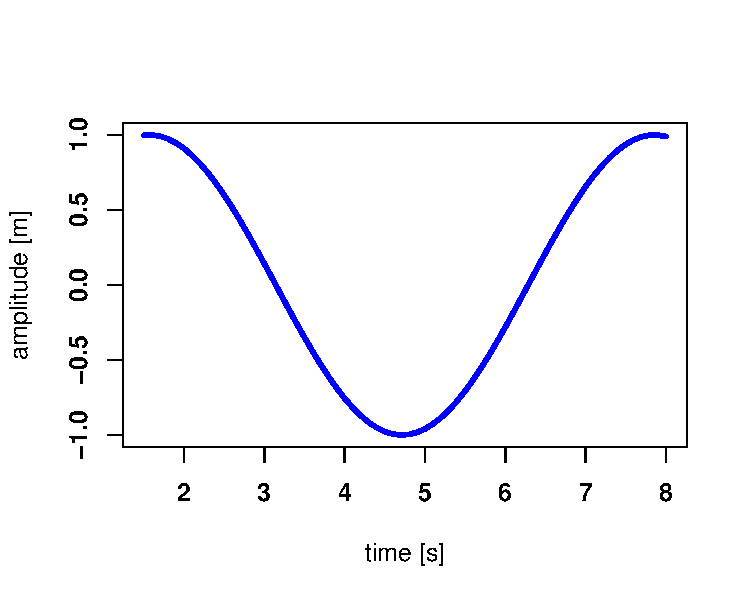
\includegraphics[width=1\linewidth]{OA_Archaeo_files/figure-latex/results-1} \caption{In-text Picture}\label{fig:results}
\end{figure}

Reference to Figure \ref{fig:results}.

\hypertarget{open-access-policy}{%
\subsection*{Open Access policy}\label{open-access-policy}}
\addcontentsline{toc}{subsection}{Open Access policy}

Based on data from SHERPA/RoMEO (new version, no more colours\ldots)

\hypertarget{one-or-two-journals-examples}{%
\subsection*{One or two journals examples}\label{one-or-two-journals-examples}}
\addcontentsline{toc}{subsection}{One or two journals examples}

The change towards OA for some big journals, maybe better from different publishers (JAS for Elsevier and the creation of JASReports? Antiquity for Cambridge? AJPA for Wiley? Journal of Archaeological Method and Theory
for Springer (the biggest Wiley in the GScholar h5 values))

\hypertarget{discussion}{%
\section*{Discussion}\label{discussion}}
\addcontentsline{toc}{section}{Discussion}

\hypertarget{conclusion}{%
\section*{Conclusion}\label{conclusion}}
\addcontentsline{toc}{section}{Conclusion}

\hypertarget{acknowledgments}{%
\section*{Acknowledgments}\label{acknowledgments}}
\addcontentsline{toc}{section}{Acknowledgments}

The authors would like to thank XXX and YYY.

\hypertarget{references}{%
\section*{References}\label{references}}
\addcontentsline{toc}{section}{References}

\hypertarget{refs}{}
\begin{cslreferences}
\leavevmode\hypertarget{ref-pourret_open_2020}{}%
Pourret, Olivier, Andrew Hursthouse, Dasapta Erwin Irawan, Karen Johannesson, Haiyan Liu, Marc Poujol, Romain Tartèse, Eric D. van Hullebusch, and Oliver Wiche. 2020. ``Open Access Publishing Practice in Geochemistry: Overview of Current State and Look to the Future.'' \emph{Heliyon} 6 (3): e03551. \url{https://doi.org/10.1016/j.heliyon.2020.e03551}.
\end{cslreferences}



\end{document}
